\documentclass[a4paper, 12pt]{article}%тип документа

%отступы
\usepackage[left=2cm,right=2cm,top=2cm,bottom=3cm,bindingoffset=0cm]{geometry}
\setlength{\parindent}{5ex}

%Русский язык
\usepackage[T2A]{fontenc} %кодировка
\usepackage[utf8]{inputenc} %кодировка исходного кода
\usepackage[english,russian]{babel} %локализация и переносы

%Вставка картинок
\usepackage{graphicx}
\graphicspath{{pictures/}}
\DeclareGraphicsExtensions{.pdf,.png,.jpg}

%Графики
\usepackage{pgfplots}
\pgfplotsset{compat=1.9}

%Математика
\usepackage{amsmath, amsfonts, amssymb, amsthm, mathtools}

%Таблицы
\usepackage{longtable} 
\usepackage{float}

%Римские цифры
\newcommand{\RomanNumeralCaps}[1]{\uppercase\expandafter{\romannumeral#1}}

\usepackage{multirow}


\begin{document}
	\begin{titlepage}
		\begin{center}
			\textsc{Федеральное государственное автономное образовательное учреждение высшего образования«Московский физико-технический институт (национальный исследовательский университет)»\\[5mm]
			}
			
			\vfill
			
			\textbf{Отчёт по лабораторной работы 3.7.1\\[3mm]
				Скин-Эффект в полом цилиндре.
				\\[50mm]
			}
			
		\end{center}
		
		\hfill
		\begin{minipage}{.5\textwidth}
			Выполнил студент:\\[2mm]
			Сериков Василий Романович\\[2mm]
			группа: Б03-102\\[5mm]
			
		\end{minipage}
		\vfill
		\begin{center}
			Москва, 2022 г.
		\end{center}
		
	\end{titlepage}
	
	\newpage
	\textbf{Аннотация}\\
	
	
	\textbf{Цель работы: }\\
	Исследование проникновения переменного магнитного поля в медный полый цилиндр.\\
	
	\textbf{В работе используются: }\\
	 Генератор звуковой частоты, соленоид, намотанный на полый цилиндрический каркас из диэлектрика, медный экран
	в виде трубки, измерительная катушка, амперметр, вольтметр, осциллограф.\\
	
	\textbf{Теоретические сведения: } \\
	Рассмотрим квазистационарное поле внутри проводящей среды в плоском случае.
	\begin{figure}[H]
		\center{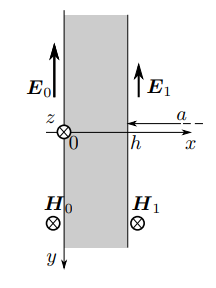
\includegraphics[scale=1]{plosk.png}}
		\caption{Скин эффект в плоской геометрии.}
	\end{figure}
	Пусть вектор ${E}$ направлен всюду вдоль оси $y$  
	и зависит только от координаты $x$, т. е. ${E_x} = {E_z} \equiv 0$, $E_y=E_y(x,t)$.
	В квазистационарном приближении 
	\begin{equation}
		\nabla \times {H} = \sigma {E}
	\end{equation}
	Берем ротор обеих частей
	\begin{equation}
		\nabla \times (\nabla \times {H}) = \nabla(\nabla \cdot {H}) - \nabla^2{H} = \sigma \nabla \times {E}
	\end{equation}
	Используя уравнение Максвелла для ротора ${E}$ и для дивергенции ${H}$ получаем
	\begin{equation}
		\nabla^2 {H} = \sigma\mu\mu_0\frac{\partial{H}}{\partial t} 
		+ \nabla(\nabla \cdot {H}) = \sigma\mu\mu_0\frac{\partial{H}}{\partial t} 
		\label{eq:laplacian_H}
	\end{equation}
	Берем ротор еще раз
	\begin{equation}
		\nabla \times (\nabla^2{H}) = \nabla^2 (\nabla \times {H}) =
		\sigma\mu\mu_0 \frac{\partial (\nabla \times {H})}{\partial t}
	\end{equation}
	Осталось подставить первое уравнение, и воспользоваться уравнением Максвелла
	\begin{equation}
		\nabla^2{E}=\sigma\mu\mu_0 \frac{\partial {E}}{\partial t}\label{eq:diffusion}
	\end{equation}
	
	Подставляем электрическое поле $E_y=E_y(x,t)$
	\begin{equation}
		\frac{\partial^2 E_y}{\partial x^2} = \sigma\mu\mu_0\frac{\partial E_y}{\partial t}
		\label{eq:diffusion_chastni}
	\end{equation}
	Если $E_y(0,t)=E_0 e^{i\omega t}$ то решением будет функция вида
	\begin{equation}
		E_y(x,t)=E_0 e^{-x/\delta} e^{i(\omega t - x/\delta)}
		\label{eq:skin_effect_poluprostranstvo}
	\end{equation}
	где
	\begin{equation}
		\delta = \sqrt{\frac{2}{\omega\sigma\mu\mu_0}}
		\label{eq:delta}
	\end{equation}
	
	\textbf{Скин-эффект в тонком полом цилиндре}
	\begin{figure}[H]
		\center{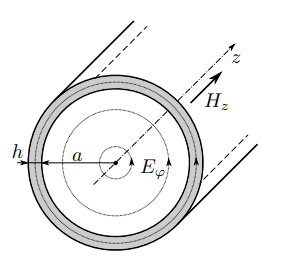
\includegraphics[scale=1]{cilindr.png}}
		\caption{ Электрическое и магнитное в тонкостенном цилиндре.}
	\end{figure}
	Из симметрии и 
	непрерывности соответствующих компонент векторов ${E}$ и ${H}$ можем сказать что
	\begin{equation}
		H_z = H(r)e^{i\omega t} \text{, } E_\varphi = E(r)e^{i\omega t}
	\end{equation}
	и при этом функции $H(r)$ и $E(r)$ непрерывны.
	
	Внутри цилиндра токов нет, следовательно $H(r)=H_1=\text{const}$ внутри цилиндра.
	По теореме об электромагнитной индукции
	\begin{equation}
		E(r) = -\frac{1}{2}\mu_0 r \cdot i \omega H_1
	\end{equation}
	откуда мы получаем граничное условие
	\begin{equation}
		E_1=E(a)= -\frac{1}{2}\mu_0 a \cdot i \omega H_1
		\label{eq:granichnoe_uslovie_E}
	\end{equation}
	
	В приближении $h \ll a$ можем пренебречь кривизной стенки и считать ее бесконечной полосой. Тогда, надо решить уравнение
	с граничными условиями. Решая уравнение получим связь полей $H_1$ 
	(поле внутри цилиндра которое мы будем измерять) и $H_2$, которое колеблется с частотой
	$\omega$
	
	\begin{equation}
		H_1 = \frac{H_0}{\ch(\alpha h) + \frac{1}{2} \alpha a \sh(\alpha h)} 
		\text{\ \ \ }
		\alpha = \sqrt{i\omega \sigma \mu_0} = \frac{\sqrt{2}}{\delta}e^{i\pi/4}
		\label{eq:svyaz_poley}
	\end{equation}
	
	из этой формулы получим сколько по фазе отстает поле $H_1$ от $H_0$. При $\delta \ll h$
	(высокочастотная область)
	
	\begin{equation}
		\psi \approx \frac{\pi}{4} + \frac{h}{\delta} = 
		\frac{\pi}{4} + h \sqrt{\frac{\omega \sigma \mu_0}{2}}
		\label{eq:faza_high_freq}
	\end{equation}
	
	При $\delta \gg h$ (низкочастотная область)
	
	\begin{equation}
		\tan \psi \approx \frac{ah}{\delta^2} = \pi a h \sigma \mu \mu_0 \nu
		\label{eq:faza_low_freq}
	\end{equation}
	
	\textbf{Экспериментальная установка: }\\
	\begin{figure}[H]
		\center{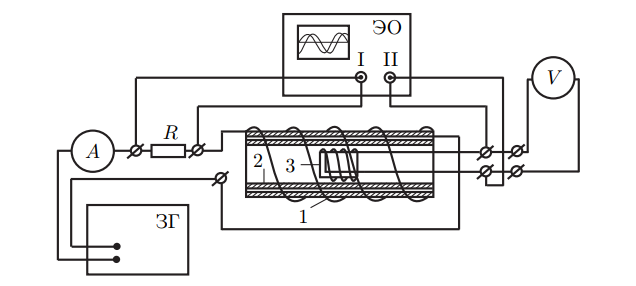
\includegraphics[scale=1]{ust.png}}
		\caption{Экспериментальная установка.}
	\end{figure}
	Схема экспериментальной установки для исследования проникновения переменного магнитного поля в медный полый цилиндр изображена
	на рис. 3. Переменное магнитное поле создаётся с помощью соленоида,
	намотанного на полый цилиндрический каркас 1 из поливинилхлорида,
	который подключается к генератору звуковой частоты. Внутри соленоида расположен медный цилиндрический экран 2. Для измерения магнитного поля внутри экрана используется измерительная катушка 3.
	Необходимые параметры соленоида, экрана и измерительной катушки
	указаны на установке. Действующее значение переменного тока в цепи
	соленоида измеряется амперметром A, а действующее значение напряжения на измерительной катушке измеряет вольтметр V . Для измерения
	сдвига фаз между током в цепи соленоида и напряжением на измерительной катушке используется двухканальный осциллограф. На вход одного
	канала подаётся напряжение с резистора R, которое пропорционально
	току, а на вход второго канала — напряжение с измерительной катушки
	
	ЭДС индукции в измерительной катушке равна
	$$
	\boldsymbol{U}=-S N \frac{d B_1(t)}{d t}=-i \omega \mu_0 S N H_1 e^{i \omega t},
	$$
	где $S N$ - произведение площади витка на число витков измерительной катушки. Показания вольтметра, измеряющего это напряжение:
	$$
	U=\frac{S N \omega}{\sqrt{2}} \mu_0\left|H_1\right| .
	$$

	$$
	\frac{\left|H_1\right|}{\left|H_0\right|}=\text { const } \cdot \frac{U}{\nu I}
	$$
	
	Таким образом, отношение амплитуд магнитных полей снаружи и зне экрана (коэффициент ослабления) может быть измерено по отношению $U / \nu I$ при разных частотах. Неизвестная константа может быть определена по измерениям при малых частотах $\nu \rightarrow 0$ $\left|H_1\right| /\left|H_0\right| \rightarrow 1$.\\
	
	
	\textbf{Результаты измерений и обработка данных: }\\
	\begin{enumerate}
		
	\item В области низких частот — от $ 0,01\nu_h \text{ до }  0,1\nu_h (\nu_h \approx 2200$ Гц)  — получим зависимость отношения $\xi = U/\nu I $ от частоты $\nu$.
	Полученные данные занесем в таблицу 1.
	
	\begin{longtable} {|c|c|c|c|c|c|c|c|c|c|c|c|c|}
		\hline
		$\nu$, Гц& 20 & 29 & 38 & 47 & 56 & 65 & 74 & 83 & 92 & 101 & 110 & 119  \\ \hline
		
		$V$, B & 0,131 & 0,194 & 0,249 & 0,301 & 0,349 & 0,393 & 0,433 & 0,469 & 0,502 & 0,531 & 0,557 & 0,580 \\ \hline
		
		$I$, мА& 467 & 464 & 460 & 456 & 450 & 444 & 438 & 432 & 426 & 420 & 414 & 409 \\ \hline
		\caption{Данные для зависимости $\xi = U/\nu I $ при $\nu \text{ от } 0,01\nu_h \text{ до }  0,05\nu_h$}
	\end{longtable}
	
	\item По результатам пункта 1 построим график зависимости $1/\xi^2 = k \nu^2$, по графику определим величину $\xi_0$ и проводимость меди $\sigma$
	
	\begin{figure}[H]
		\center{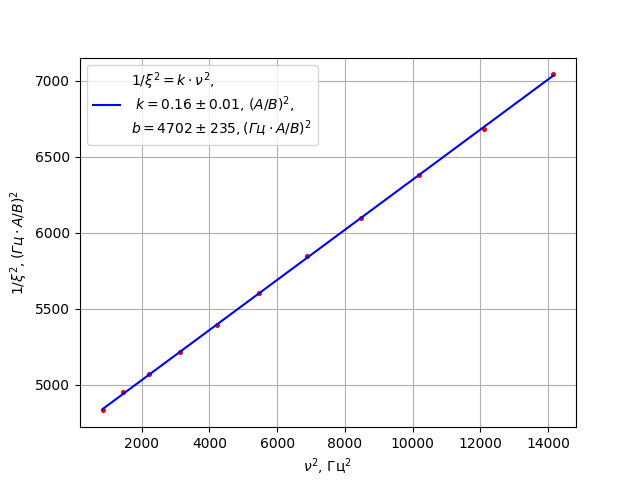
\includegraphics[scale=0.9]{3-7-1_xi2(nu2).png}}
		\caption{График зависимости $1/\xi^2 = k \nu^2$.}
	\end{figure}

	$$ \sigma^2 = \frac{(\xi_0/\xi)^2 - 1}{(ah\mu_0\pi\nu)^2} $$
	$ \sigma_{min} =  1,5 \pm 0,1$ См/м
	$ \sigma_{max} =  5,1 \pm 0,1$ См/м
	
		\newpage
		
	\item Исследуем зависимость величины $\xi$ и фазового сдвига $\psi$ от частоты
	$\nu$ при низких частотах в диапазоне от $0,05\nu_h \text{ до }  0,5\nu_h$. Полученные данные занесем в таблицу 2.
	
	\begin{longtable} {|c|c|c|c|c|c|c|c|c|c|c|}
		\hline
		$\nu$, Гц& 100 & 112 & 124 & 136 & 148 & 160 & 172 & 184 & 196 & 220  \\ \hline
		
		$V$, B & 0,526 & 0,561 & 0,590 & 0,616 & 0,637 & 0,656 & 0,672 & 0,686 & 0,697 & 0,716 \\ \hline
		
		$I$, мА& 419 & 411 & 404 & 397 & 391 & 386 & 381 & 376 & 372 & 364  \\ \hline
		
		$\psi$, $^\circ$ & 68 & 56 & 54 & 53,5 & 47,7 & 46,5 & 45 & 41,5 & 36 & 32,7   \\ \hline
		\hline
		\hline
		
		$\nu$, Гц & 305 & 390 & 475 & 560 & 645 & 730 & 815 & 900 & 985 & 1070   \\ \hline
		
		$V$, B  & 0,752 & 0,763 & 0,764 & 0,759 & 0,752 & 0,742 & 0,730 & 0,717 & 0,703 & 0,688  \\ \hline
		
		$I$, мА& 347 & 335 & 327 & 320 & 313 & 307 & 301 & 295 & 288 & 282  \\ \hline
		
		$\psi$, $^\circ$ & 28,1 & 22,8 & 19,6 & 16,4 & 11,8 & 11,0 & 9,0 & 8,2 & 3,6 & 0  \\ \hline
		
		\caption{Данные для $V, I, \psi$}
	\end{longtable}	
	\item Построим график зависимости фазового сдвига от частоты $\tg \psi = f(\nu)$. Определим участок, где есть линейная зависимость и по наклону прямой определим коэффициент проводимости.
	
	\begin{figure}[H]
		\center{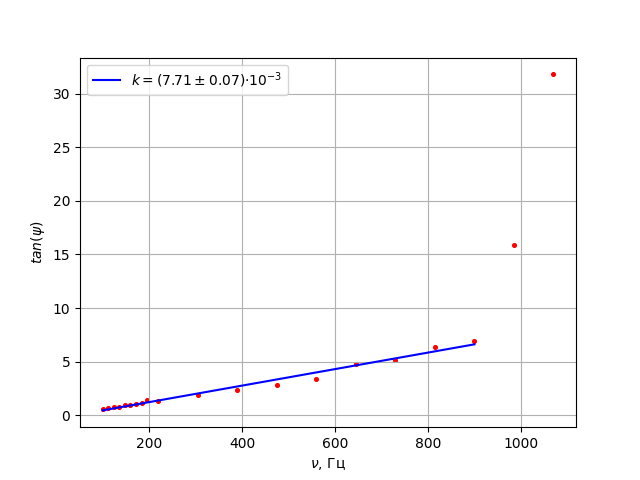
\includegraphics[scale=0.9]{3-7-1_tan(psi)(nu).png}}
		\caption{График зависимости $\tg(\psi) = f(\nu)$.}
	\end{figure}

	$$ \sigma = \frac{k}{ah\pi\mu_0} = (5,8 \pm 0,3)\cdot 10^7 \text{См/м}$$
	
	\newpage
		
	\item Повторим измерения пункта 3 при высоких частотах в диапазоне $ \text{ от } 0,5\nu_h \text{ до } 15\nu_h$. Полученные данные занесем в таблицу 3.
	
	\begin{longtable} {|c|c|c|c|c|c|c|c|c|c|c|}
		\hline
		$\nu$, кГц& 1,1 & 3,3 & 5,5 & 7,7 & 9,9 & 12,1 & 14,3 & 16,5 & 18,7 & 20,9  \\ \hline
		
		$V$, B & 0,683 & 0,368 & 0,224 & 0,151 & 0,108 & 0,081 & 0,062 & 0,049 & 0,040 & 0,034 \\ \hline
		
		$I$, мА& 279 & 153 & 99 & 71 & 55 & 43 & 35 & 28 & 23 & 19  \\ \hline
		
		$\psi$, $^\circ$ & 0 & 24,2 & 36 & 51,2 & 72,3 & 90,0 & 101,3 & 115,7 & 135,0 & 140,9  \\ \hline
		
		\hline
		\hline
		
		$\nu$, кГц & 23 & 25 & 28 & 30 & 32 &  &  &  &  &    \\ \hline
		
		$V$, B  & 0,029 & 0,025 & 0,021 & 0,017 & 0,013 &  &  &  &  &   \\ \hline
		
		$I$, мА& 14,5 & 11,0 & 7,8 & 4,9 & 2,7 &  &  &  &  &   \\ \hline
		
		$\psi$, $^\circ$ & 145,7 & 160,0 & 161,1 & 168,1 & 191,6 &  &  &  &  &   \\ \hline
		
		\caption{Данные для зависимости $\xi = U/\nu I $ и $\psi$ при $\nu \text{ от } 0,05\nu_h \text{ до }  0,5\nu_h$}
	\end{longtable}	

	\item Построим график частотной зависимости фазового сдвига $\psi - \pi/4 = f(\sqrt{\nu})$ для данных из пунктов 3 и 5. Проведем прямую, проходящую через начало координат, которая будет касаться линейного участка графика. По наклону прямой определим проводимость материала экрана.
	
	\begin{figure}[H]
		\center{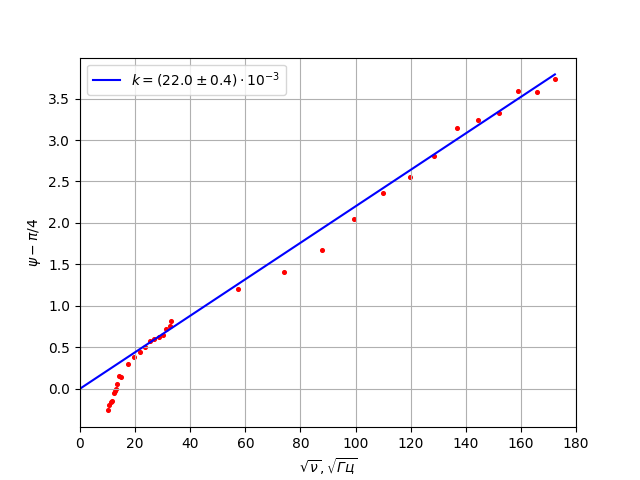
\includegraphics[scale=0.9]{3-7-1_psi(nu).png}}
		\caption{График зависимости $\psi - \pi/4 = f(\sqrt{\nu})$.}
	\end{figure}

	$$ \sigma = \frac{k^2}{\pi \mu_0 h^2} = (5,4 \pm 0,2)\cdot 10^7 \text{См/м} $$
	
	\item Исследуем зависимость индуктивности катушки $L$ от частоты $\nu$. Полученные данные занесем в таблицу 4.
	
		\begin{longtable} {|c|c|c|c|c|c|c|c|c|c|c|}
		\hline
		$\nu$, Гц& 50 & 150 & 250 & 400 & 500 & 600 & 750 & 800 & 1000 & 1500  \\ \hline
		
		$L$, мГн & 10,38 & 7,55 & 5,68 & 4,27 & 3,86 & 3,62 & 3,40 & 3,35 & 3,22 & 3,09 \\ \hline
		
		\hline
		\hline
		
		$\nu$, Гц & 4000 & 5000 & 7500 & 10000 & 15000 & 16200 & 20000 &  &  &    \\ \hline
		
		$L$, мГн  & 0,12 & 3,03 & 3,07 & 3,15 & 3,47 & 3,58 & 4,1 &  &  &   \\ \hline
		
		\caption{Данные для зависимости $L(\nu)$ при $\nu \text{ от } 0,02\nu_h \text{ до }  10\nu_h$}
	\end{longtable}	
		
	
	\item Построим график зависимости индуктивности катушки от частоты $L(\nu)$. Определим максимальное и минимальное значение индуктивности.
	
	\begin{figure}[H]
		\center{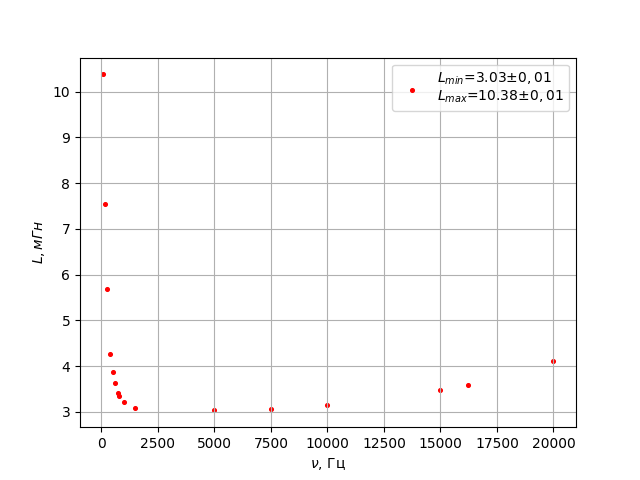
\includegraphics[scale=0.9]{3-7-1_L(nu).png}}
		\caption{График зависимости $L(\nu)$.}
	\end{figure}
	
	\newpage
	
	\item Построим график зависимости $(L_{max} - L_{min})/(L - L_{min})(\nu^2)$, по наклону определим проводимость материала экрана
	
	\begin{figure}[H]
		\center{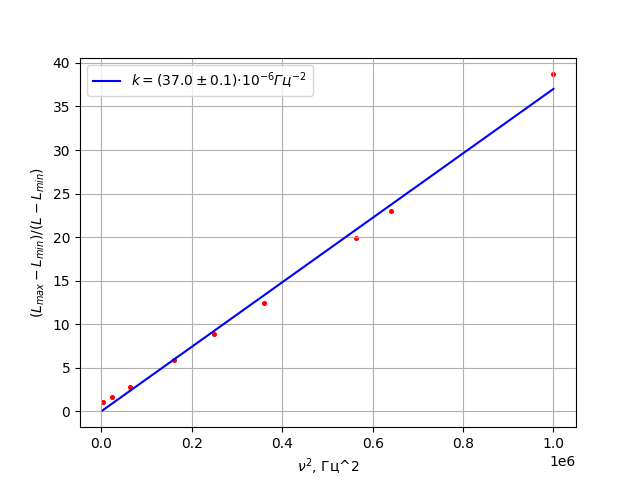
\includegraphics[scale=0.9]{3-7-1_L(nu2).png}}
		\caption{График зависимости $(L_{max} - L_{min})/(L - L_{min})(\nu^2)$.}
	\end{figure}

	$$ \sigma = \frac{\sqrt{k}}{\pi a \mu_0 h} = (5,0 \pm 0,3)\cdot 10^7 \text{См/м} $$
	
	\newpage
	
	\item По полученному коэффициенту $\xi_0$ определим коэффициенты ослабления поля $ |H_1|/|H_0|$. Изобразим на графике зависимость $ |H_1|/|H_0|$ от  $\nu$ в логарифмическом масштабе. Также построим теоретическую кривую.
	
	\begin{figure}[H]
		\center{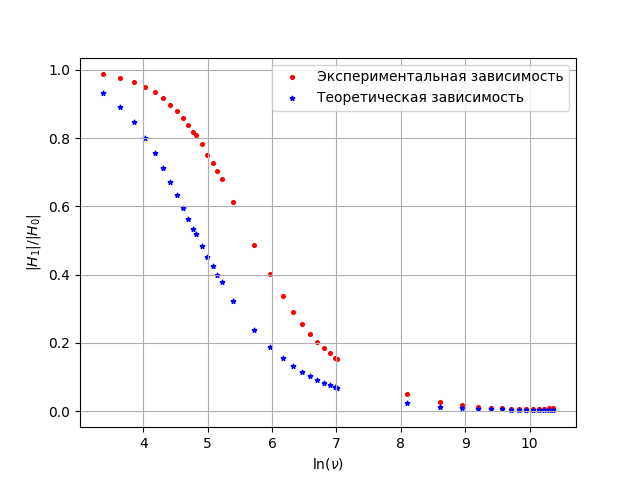
\includegraphics[scale=0.9]{3-7-1_H(ln(nu)).png}}
		\caption{График зависимости $|H_1|/|H_0|(ln(\nu))$.}
	\end{figure}
	
	
		
	\end{enumerate}
	
	
	
	\textbf{Обсуждение результатов и выводы: }\\
	
	\begin{longtable} {|c|c|}
		\hline
		$\sigma$, $\cdot 10^7$ См/м & $\varepsilon$, \% \\ \hline
		1,5 - 5,1 & 2 \\ \hline
		5,8 & 5 \\ \hline
		5,4 & 4 \\ \hline
		5,0 & 6 \\ \hline
		\caption{Сводная таблица всех полученных результатов}
	\end{longtable}
	
	В ходе данной работы мы исследовали проникновение переменного магнитного поля в медный полый цилиндр. Получили значение проводимости меди различными способами. Теоретическое значение проводимости меди: $\sigma = 5-6 \cdot 10^7$ См/м. Полученные нами значения совпадают в пределах погрешности с теоретическим. Также мы определили коэффициенты ослабления поля и измерили индуктивность катушки цилиндра, все полученные данные отобразили на графиках.
	
	
	
	
	
	
	
	
	
	
	
	
	
	
	
	
	
	
	
	
	
	
	
	
	
	
	
	
	
	
	
	
	
	
	
	
	
	
	
	
	\end{document}